\documentclass[a4paper,12pt]{article}
\usepackage[utf8]{inputenc}
\usepackage[T1]{fontenc}
\usepackage{graphicx}

\usepackage{caption}
\usepackage{amsmath}
\usepackage{hyperref}

\title{Analisi Comparativa del Clustering di Risposte LLM con BERT Fine-Tuned e BERT Base}
\author{Autore: \emph{Il Tuo Nome}\thanks{Email: tuonome@esempio.com}}  
\date{\today}

\begin{document}
\maketitle

\begin{abstract}
In questo lavoro conduciamo un'analisi comparativa tra due pipeline di estrazione e clustering di embedding di risposte generate da LLM. Nel primo esperimento (Run A), utilizziamo un modello \textit{BERT-base} fine-tuned per distinguere risposte "jailbreak" da risposte regolari; nel secondo (Run B), impieghiamo il medesimo modello BERT-base in versione non fine-tuned. Entrambi i set di embedding vengono raggruppati tramite K-Means (\(k=2\)) e visualizzati mediante PCA e t-SNE. Confrontiamo distribuzioni, separabilità e compattezza dei cluster per valutare l'effetto del fine-tuning sulla rappresentazione vettoriale.
\end{abstract}

\section{Introduzione}
La crescente diffusione di modelli di linguaggio di grandi dimensioni (LLM) impone la necessità di identificare automaticamente risposte indesiderate, ad esempio tentativi di jailbreak. In letteratura, l'addestramento supervisionato di un classificatore su esempi annotati migliora la discriminazione; tuttavia, è interessante capire come il fine-tuning influisca sulla struttura degli embedding stessi. Il presente studio si concentra sul confronto tra embedding estratti da un BERT-base fine-tuned e un BERT-base non fine-tuned, usando clustering non supervisionato.

\section{Metodologia}
\subsection{Dataset e Pre-elaborazione}
Le risposte LLM analizzate (\texttt{response.json}) comprendono sia esempi di jailbreak sia risposte conforme alle policy. Nessuna ulteriore normalizzazione è applicata al testo: ogni risposta è tokenizzata con il tokenizer di BERT.

\subsection{Modelli di Embedding}
\begin{itemize}
  \item \textbf{Run A (BERT Fine-Tuned):} modello \texttt{Teto03/Bert_base_fineTuned} (2 classi) caricato tramite \texttt{AutoModelForSequenceClassification}. L'output utilizza lo stato nascosto del token [CLS] dell'ultimo layer.
  \item \textbf{Run B (BERT Base):} modello pre-addestrato \texttt{bert-base-uncased}, caricato tramite \texttt{BertModel}, senza ulteriori personalizzazioni; estrazione identica del vettore [CLS].
\end{itemize}

\subsection{Clustering e Visualizzazione}
Per entrambi i run, i vettori [CLS] vengono raggruppati con K-Means (\(k=2\), \(\mathrm{random\_state}=42\)). La separazione dei cluster è rappresentata con:
\begin{enumerate}
  \item PCA (2 componenti principali) per una panoramica lineare.
  \item t-SNE (2D, \textit{perplexity}= \(\min(30,n\!\_samples-1)\)) per un embedding non lineare ad alta risoluzione.
\end{enumerate}
Le figure~\ref{fig:pca_tuned}--\ref{fig:tsne_untuned} presentano rispettivamente PCA e t-SNE per i due esperimenti.

\section{Risultati}
\subsection{Distribuzione dei Cluster}
La Tabella~\ref{tab:distribuzione} riporta la ripartizione delle risposte nei due cluster.

\begin{table}[h]
  \centering
  \caption{Distribuzione dei risposte per cluster nei due esperimenti}
  \label{tab:distribuzione}
  \begin{tabular}{lrrr}
    \hline
    \textbf{Modello} & \textbf{Cluster} & \textbf{Conteggio} & \textbf{Percentuale} \\
    \hline
    BERT Fine-Tuned & 0 & 1087 & 61.31\% \\
                    & 1 &  686 & 38.69\% \\
    BERT Base      & 0 &  331 & 18.67\% \\
                    & 1 & 1442 & 81.33\% \\
    \hline
  \end{tabular}
\end{table}

\subsection{Visualizzazioni PCA}
\begin{figure}[h]
  \centering
  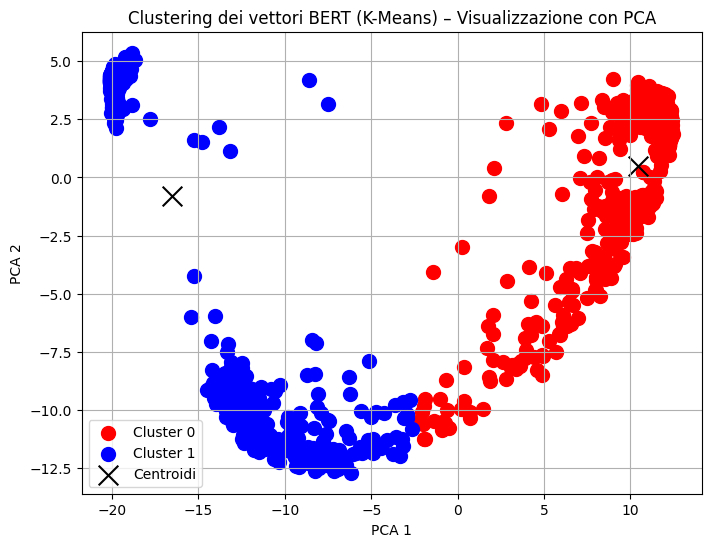
\includegraphics[width=0.8\textwidth]{1.png}
  \caption{PCA dei cluster estratti dal BERT Fine-Tuned (Run A).}
  \label{fig:pca_tuned}
\end{figure}

\begin{figure}[h]
  \centering
  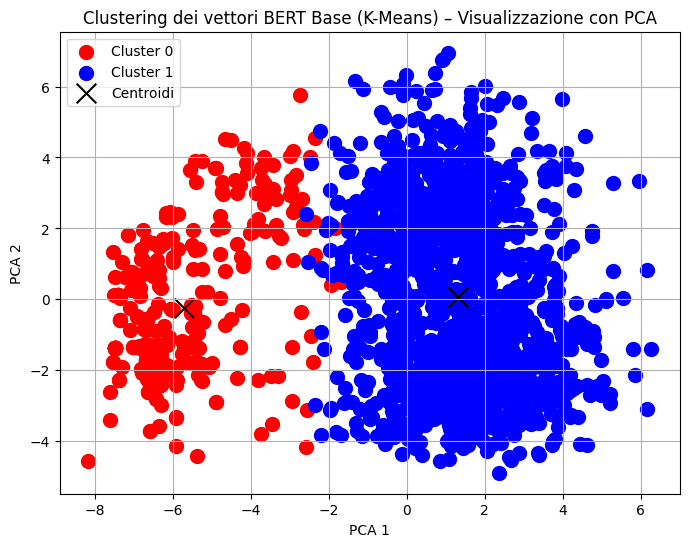
\includegraphics[width=0.8\textwidth]{3.png}
  \caption{PCA dei cluster estratti dal BERT Base (Run B).}
  \label{fig:pca_untuned}
\end{figure}

\subsection{Visualizzazioni t-SNE}
\begin{figure}[h]
  \centering
  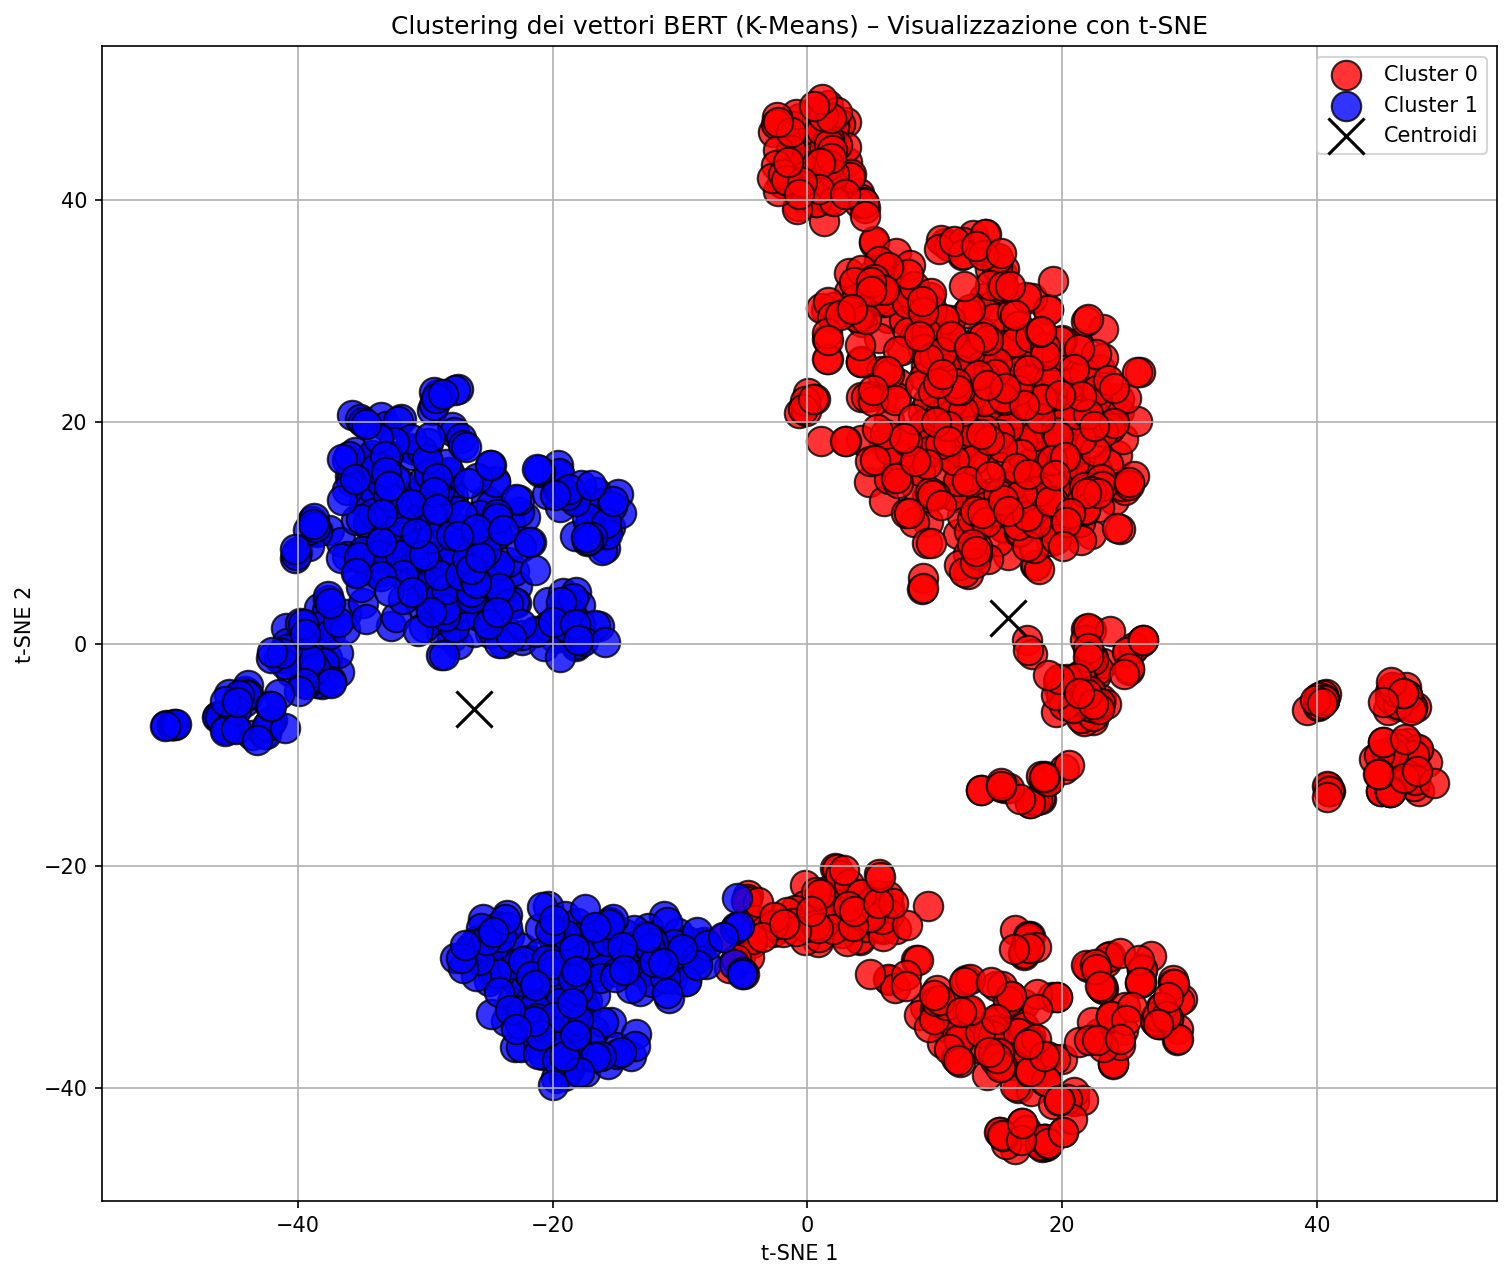
\includegraphics[width=0.8\textwidth]{2.png}
  \caption{t-SNE dei cluster estratti dal BERT Fine-Tuned (Run A).}
  \label{fig:tsne_tuned}
\end{figure}

\begin{figure}[h]
  \centering
  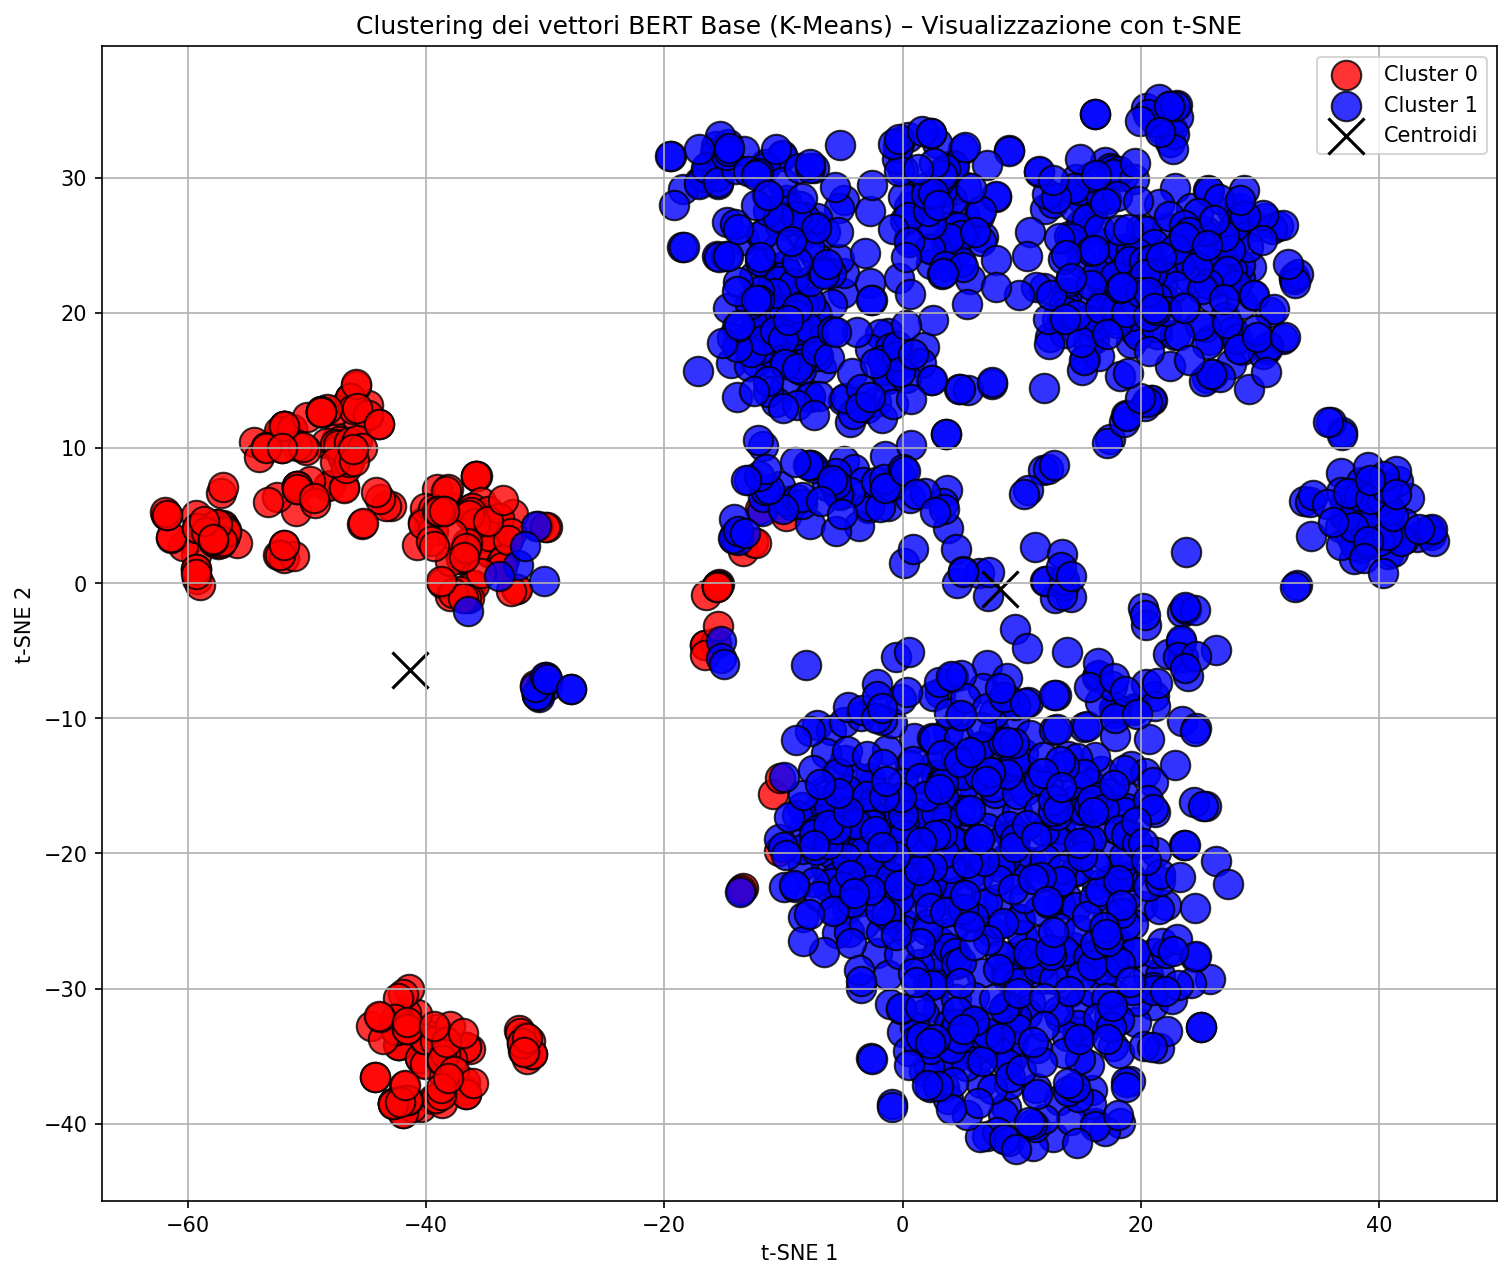
\includegraphics[width=0.8\textwidth]{4.png}
  \caption{t-SNE dei cluster estratti dal BERT Base (Run B).}
  \label{fig:tsne_untuned}
\end{figure}

\section{Discussione}
L'analisi mostra differenze sostanziali nella distribuzione e nell'organizzazione degli embedding:
\begin{itemize}
  \item \textbf{Distribuzione:} il modello fine-tuned assegna maggiormente le risposte al Cluster~0 (61\%), suggerendo che la rete personalizzata riconosce un gruppo consistente di esempi con caratteristiche comuni (presumibilmente jailbreak). Il BERT base invece concentra l'81\% nel Cluster~1, evidenziando un bias dell'embedding non addestrato verso una sola regione dello spazio.
  \item \textbf{Separabilità:} le visualizzazioni PCA e t-SNE di Run A appaiono più nitide e con cluster ben distinti, specialmente in t-SNE (Figura~\ref{fig:tsne_tuned}), che presenta due nuvole compatte e minor overlap. Run B, pur mostrando due raggruppamenti, rivela sovrapposizioni maggiori e densità meno omogenee.
  \item \textbf{Compattezza dei Cluster:} i centroidi di Run A sono più distanti l'uno dall'altro in entrambe le proiezioni, indicando embedding più discriminativi, mentre in Run B la distanza inter-centroide risulta inferiore.
  \item \textbf{Implicazioni pratiche:} un modello fine-tuned fornisce embedding più adatti a separare categorie di risposta rilevanti per la sicurezza; l'embedding non fine-tuned, non progettato per tale compito, porta a raggruppamenti meno informativi.
\end{itemize}

\section{Conclusioni}
Il fine-tuning di BERT sulle risposte jailbreak incrementa significativamente la qualità degli embedding per il task di distinzione non supervisionata, come evidenziato da distribuzioni più bilanciate e cluster più separati. Questi risultati suggeriscono l'opportunità di adottare modelli specificamente addestrati quando si desidera applicare tecniche di clustering per l'analisi di contenuti LLM in ambienti di produzione.

\end{document}

